\section{Approach to Managing HW/SW Interface Traceability Links}
\label{sec:approach}

%In this section, we first present an overview of our framework. We then propose the underlying data model. After that, we focus on how we design the anchors in the code and specification, which are utilized in the data model to capture traceability links.
%
%\subsection{Overview}
%\todo{this section need rewriting. focus on data.}
%\begin{figure}
%\begin{center}
%\includegraphics[width=0.55\textwidth]{framework}
%\caption{Framework of Our Approach.}
%\label{fig:framework}
%\end{center}
%\end{figure}
%
%As shown in Figure~\ref{fig:framework}, the framework of our approach consists three components: database, control logic, and user interface. The structure of the traceability link data in the database is defined by the data model. Control logic lays in the middle of user interface and datamodel. It receives and processes command from the user interface. Depending on the command, it either updates the database, or queries the data in the database and report the result to the user interface. User interface is responsible of communicating with the end user, processs and passes the input from user to the control logic, get the result from the control logic and present the result to the user.

We have developed a framework for managing traceability links between specification and implementation of HW/SW interfaces.
This framework supports fine-grained links between basic elements of specifications and constructs of implementation languages 
and automatic migration of valid traceability links as implementation evolves. Central to this framework is a simple, but 
effective data model for organizing the data of the traceability links. In support of this data model, we have identified 
anchors in implementation and specification, which identify the pieces of specification and code involved in traceability 
links. The data model with these anchors fulfills the three requirements for HW/SW interface traceability links identified above.
In this section, we first introduce the data model and then discuss the design of anchors in code and spec.  

\subsection{Data Model}
The data model is central to support fine-grained links between basic elements of specifications and constructs of implementation languages and automatic migration of links as implementations evolve. We introduce the data model of our approach in this section.

\begin{figure}
\begin{center}
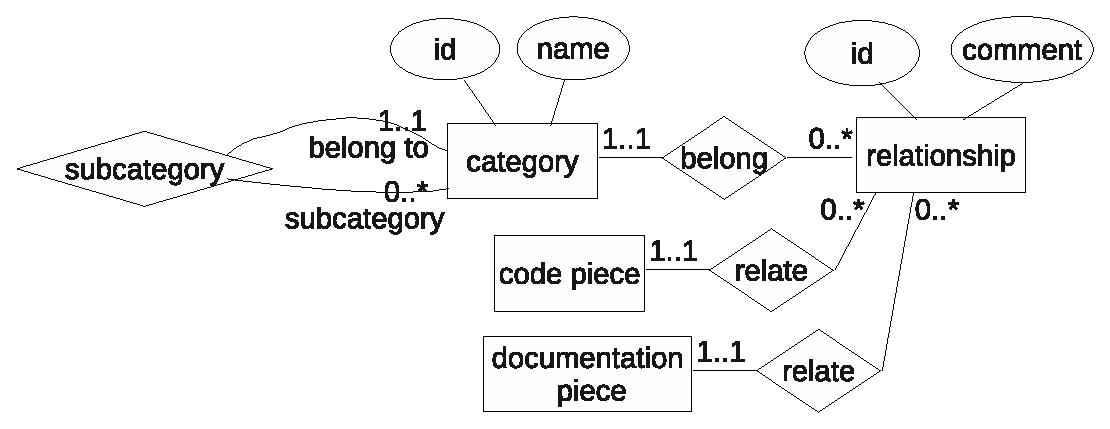
\includegraphics[width=0.85\textwidth]{datamodel}
\caption{Data Model. Entity-Relation Model is used: rectangles represent entity sets; ovals represent attributes; diamonds represent relationships.}
\label{fig:datamodel}
\end{center}
\end{figure}

The data model describes the data objects being handled in the framework, their attributes, and the relationships between these data objects.
Figure~\ref{fig:datamodel} presents the data model of our design.
Entity-relationship model is used.
Rectangles represent entity sets.
Ovals represent attributes.
Diamonds represent relationships.
We have four entity sets in our design: code file mark, spec file mark, code piece anchor and specification piece anchor.
Code piece anchor and specification piece anchor represent the selected code and specification pieces respectively.
Both code file mark and spec file mark entities have attributes id and path:
id is a 128-bit number, and serves as the key of the entity;
path is the file path pointing to a file in the local machine. % not a key, it may change
Code piece anchor and spec piece anchor have id and path as attributes:
id is a 128-bit number, and serves as the key;
path points to the code or spec piece.
Traceability links are represented by the relationships between code piece anchor and spec piece anchor.

Special attention should be paid to four attributes: path for code file, path for spec file, path for code piece anchor and path for spec piece anchor.
These four attributes are foreign keys used to refer to data that is not in the database.
As foreign keys, these attributes should be able to uniquely identify the entities they refer to.
The path provided by the file system is a solution to the path for code files and spec files, as we can easily identify both code files and spec files by these pathes.
The design of the anchors in the code and spec files is key to fine-granularity and link migration. We discuss it next.
%The pathes for anchors are challenging, little work has been done to address this problem.

%Based on the model above, we can conclude the schema as following.
%Examples?

%\subsection{Anchor Design}
%
%Anchors include specification anchor and implementation anchor. The three basic requirements for traceability links are the constraints for the design. We present how our approach fulfilled these requirements. Specification anchor design is addressed first, then we present the implementation anchor design.

\subsection{Design of Spec Anchor}

Specifications are relatively stable, which make the specification anchor design easier than implementation anchor. Using the absolute coordinate is enough to meet the requirements. Most of the HW/SW interface specification are in PDF format. We use this format to present our approach. Basically, the coordinate for specification piece is denoted by two points -- the point representing the beginnings of the selection and the point representing the end of the selection. Each point is denoted by a vector $<$page, x-coord, y-coord$>$, where page is the page number the point located, x-coord and y-coord are the horizontal and vertical coordinates respectively.

The method is accurate as each point is uniquely represented by the coordinate. This method is also fine-grained, because this method could represent each word, sentence or even arbitrary size of POS. The method is not robust as it uses the absolute coordinate as the basic element of the anchor. However, specifications are relatively stable, which makes this approach acceptable.


\subsection{Design of Code Anchor}

In designing code anchors, we first experimented with offset-based anchors and syntax-tree-based anchors. We then designed hybrid anchors that integrate the above two types of anchors and address their respective limitations. 

\subsubsection{Offset-Based Anchor.}

Similar to specification anchor,
absolute coordinates can also be used as implementation anchors.
Basically, implementation code is just a string of ASCII characters.
Each piece of code is a substring of this string.
We can use the offset of the substring in the string and the length of the piece of code to represent this piece of code.
The pair (offset, length) is called Offset-Based Anchor.
Figure~\ref{fig:code}(a) illustrate this technique.
The parenthesized number in front of each line represent the offset of the first character of that line.
Using this approach, we can get the Offset-Based Anchors for the three code pieces labeled 1, 2 and 3 as (590, 4), (614, 4) and (635, 4) respectively.

The advantage of this technique is obvious, it is simple and provides fine-grained traceability. The disadvantage of this technique is that these anchors fail after the code evolves. Figure~\ref{fig:code}(b) is the code after the code in Figure~\ref{fig:code}(a) evolves. We can see the anchors we get above do not point to the previous pieces of code anymore. The reason is that such anchor depends on the number of characters preceding the piece of code. One way to overcome this limitation is to use the code information to update these links. However, such information is not always available. Most of the time, code is changed by other people. We can only get the changed code without knowing how the change was made, without fully comprehending the code.

% a figure example
\begin{figure}[h!]
  \begin{center}
    \begin{tabular}{c}
\begin{minipage}[b]{\linewidth}
  \centering
  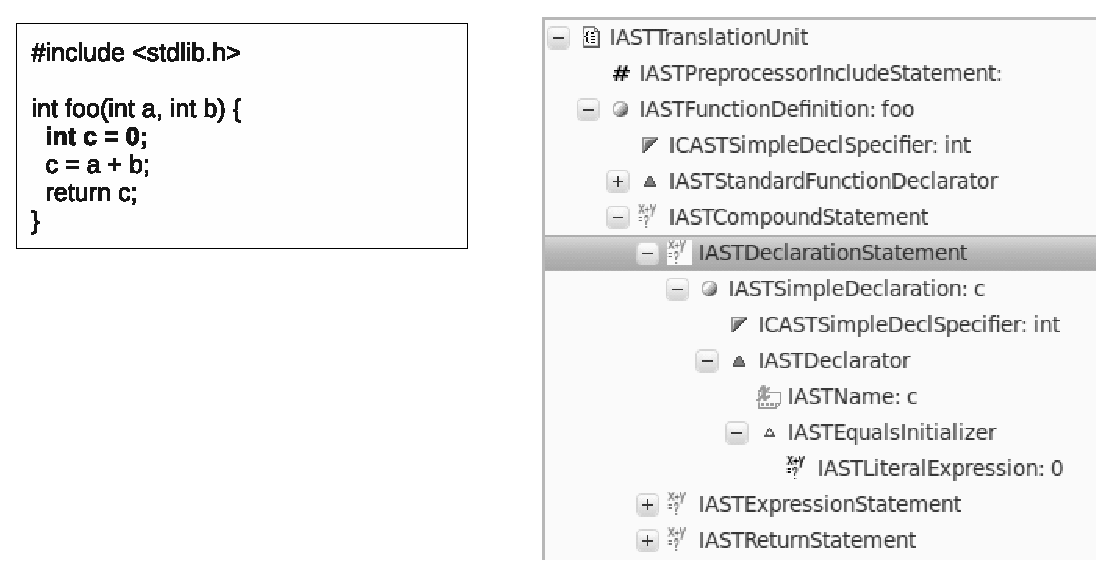
\includegraphics[width=0.8\linewidth]{ast1}
\end{minipage}\\
(a) AST for the Code in Figure~\ref{fig:code}(a)\\
\\
\begin{minipage}[b]{\linewidth}
  \centering
  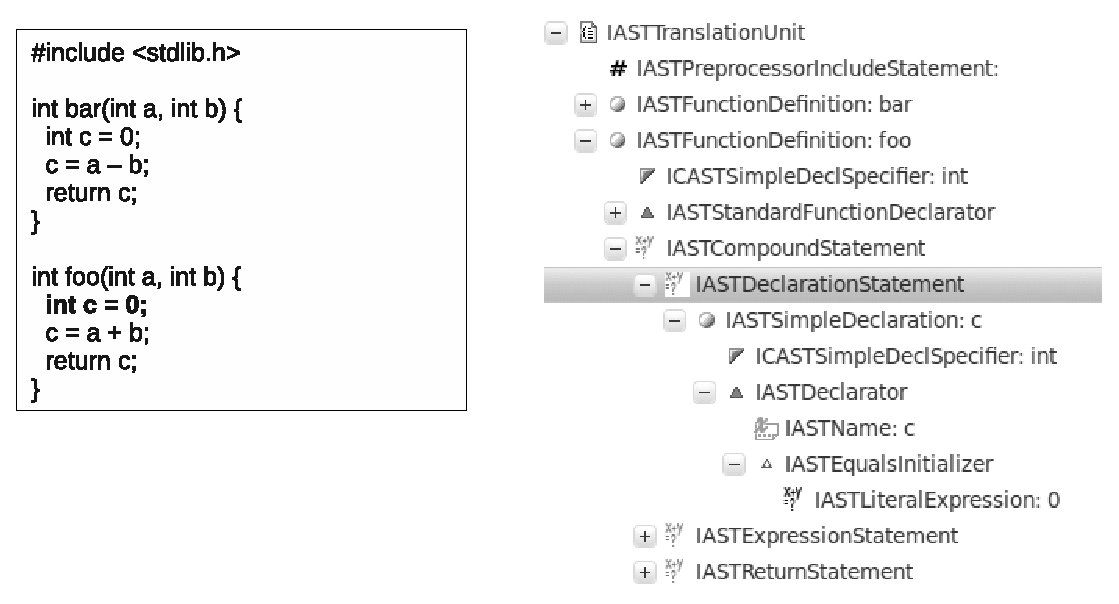
\includegraphics[width=0.8\linewidth]{ast2}
\end{minipage}\\
(b) AST for the Code in Figure~\ref{fig:code}(b)\\
\\
\begin{minipage}[b]{\linewidth}
  \centering
  \includegraphics[width=0.95\linewidth]{ast_legend}
\end{minipage}
\end{tabular}
\caption{The AST for the implementation code in Figure~\ref{fig:code}.}
\label{fig:ast}
\end{center}
\end{figure}

% syntax tree, a string of syntax tree leaf nodes.
% content-free (make immune from change of the content) vs content-sensitive (make unique)
% evaluate on unique
\subsubsection{Syntax Tree Based Anchor.}
To make the traceability links created for one version of code work for other versions,
we need a robust strategy to represent the code pieces.
More specifically, we need to find some properties of the code that are relatively stable when code evolves.
These properties can serve as keys to identify the code piece.
We use syntax information to form the main element of our code piece identifier.
The code can be parsed and represented by a parse tree or an abstract syntax tree (AST).
We use AST in our approach, as it faithfully retains the structure of the original source code, and is concise and efficient to compute compared to parse tree.
AST usually has fewer nodes than parse tree, and takes less time to traverse.
Each node in AST tree represents a syntax unit of the grammar,
a parent of a node represent a bigger grammar unit that includes the grammar unit represented by the child node.
The nodes are labeled by the type of the grammar unit.
Each leaf node includes the code this node represents in its label.
For some of the inner nodes that have a name, we also include the name in their labels. For example, an inner node that represents a function will be labeled with the grammar unit type and the name of the function.
A change of the code in one branch of AST usually does not affect the structure in other branches.
Representing code pieces based on the structure in the syntax tree is robust.
Figure~\ref{fig:ast}(a) and Figure~\ref{fig:ast}(b) are the Abstract Syntax Trees (AST) for the code in Figure~\ref{fig:code}(a) and Figure~\ref{fig:code}(b).
Dot lines represent branches not shown.
Figure~\ref{fig:ast}(a) shows two subtrees of the root.
The left subtree represents line 13 - line 25 of Figure~\ref{fig:code}(a), which defines the structure max7310\_s.
The right subtree represent line 27 - line 35 of Figure~\ref{fig:code}(a), which defines the function max7310\_reset.
Similarly, the left subtree of the AST in Figure~\ref{fig:ast}(b) represent line 12 - line 24 in Figure~\ref{fig:code}(b), and the right subtree represents line 26 - line 34.
From the AST shown in Figure~\ref{fig:ast}(a) and Figure~\ref{fig:ast}(b), we can see that the left tree has changed as the code for structure definition changed.
However, the structure of the right subtree remain the same, unaffected by the change of the left subtree.

Based on the AST of the code, we define our identifier to a piece of code as a sequence of leaf nodes in the AST. Each leaf node is represented by the path from the leaf node to the root of the AST. For example, line 31 in Figure~\ref{fig:code}(a) is represented by the highlighted three leaf nodes in Figure~\ref{fig:ast}(a). The leaf nodes are in the same order as they are visited by depth-first search of the AST. For this example, the closest common parent node for these three leaf nodes also represents the same piece of code, and this representation is even simpler. We avoid using this representation for two reasons: First, this representation contains less information; Second, this representation is sensitive to formatting and style convention. For example, some programmer may prefer no spaces adjacent to the equal sign, or they may insert some spaces besides the equal sign to make it aligned with other lines of assignment statements. Either case will change the string represented by this common parent, and make the traceability link invalid. We will address how we determine if a traceability link is valid or not in the next section.

Using this approach, consider the pieces of code labeled by 1, 2 and 3 in Figure~\ref{fig:code} again. The identifiers for these code pieces in AST are shown in Figure~\ref{fig:ast} labeled with the same numbers.
Though the two ASTs are different,
the highlighted nodes can be represented by the same paths from the roots in both ASTs.
This method can identify the piece of code and the change of the unrelated code does not invalidate the identifier.

This method is robust. However, it may not uniquely identify a piece of code, i.e., one identifier may refer to two or more pieces of code.
The pieces of code labeled 1 and 3 in Figure~\ref{fig:ast}(a) have different paths from the root of the syntax, however that have the same 
identifier -- $<$\texttt{LE:0xff/BE/ES/CS/FD:max7310\_reset/TU}$>$. As a result, such identifier cannot distinguish these two pieces of code. 

\subsubsection{Hybrid Anchor.}

Offset-based anchor can uniquely identify a piece of code, but it is not immune to code evolution.
Syntax tree based anchor is immune to code evolution, but it cannot uniquely identify pieces of code.
We combine these two methods and form hybrid anchor.
For each leaf node that has an ambiguous path representation,
we can always find at least one of its ancestors that has an unique path.
In the worst case, we will get to the root node.
Our approach is composed of two steps.
First, we compute the syntax tree based anchor, go over the path from leaf to root, and find the first node that is a unique identifier.
Second, we compute offset based anchor using this unique identifier instead of the beginning of the whole implementation code.
Consider the AST in Figure~\ref{fig:ast}(a), to identify the piece of code labeled by 1,
we go through the path towards the root,
and get to the first unique identifier at the inner node CS.
The node CS represents line 28 - line 35 of the code in Figure~\ref{fig:code}(a).
It is the body of the function \texttt{max7310\_reset}, and there is only one body for this function by the C language grammar.
The offset based identifier based on this node is (103,4), as the first character of the node CS is located at offset 487 and the offset based anchor is (590,4).
We combine the information of the inner node CS and the calculated coordinate to represent the piece of code with no ambiguity.
Same as offset based anchor, if the code does not change, it can uniquely identify the piece of code.
If the code changes, this method still works if the code identified by the unique identifier remains the same.
Actually, this is a generalization of the previous two approaches.
If we get to the root node while finding the first unique ancestor, then this approach will become the same as offset based anchor.
However, if the lead node itself is the first node with unique identifier, then this approach is the same as syntax based anchor.
The lower the node with the unique identifier in AST, the better our approach works.
%However, this method provide redundant information, which can be used to check the validity.

% example?
